The 11-city governance target has 160 city-quarters in its full observation
window.  Eight city-quarters have no compatible weeks and therefore have
missing outcome ratios; lines break at these missing observations rather than
interpolating across them.  A source-coded-zero share is the fraction of
compatible weekly records coded zero, not a verified zero-transaction rate.
Block summaries average defined quarterly ratios within their city-quarter
support rather than pooling weekly records.  The three panels retain the
outcome variables, calendar ordering, missing segments and observation-state
coding used by the governance comparison.

Figures~\ref{fig:si_city_paths_1}, \ref{fig:si_city_paths_2} and
\ref{fig:si_city_paths_3} provide the city-level check on the aggregate
governance contrasts: each page aligns $A$, $N$, $I$ and observation status on
the same relative-time axis.  Circles mark the three outcome series; in the
observation column, black circles denote time coverage and orange squares the
source-coded-zero share.  Grey shading marks a policy-transition quarter and
the dashed vertical line marks $h=0$; missing city-quarters break the lines.
These event markers orient the comparison but do not assign observed changes to
a policy.

The plotted trajectories also show why a window average can combine different
level and timing patterns.  For Haikou, $A$ rises from about 47,642 at $h=-8$
to 176,178 at $h=0$ while $N$ rises from 84.7 to 810.1 and $I$ falls from
562.5 to 217.5.  Fuzhou has missing outcome ratios at $h=-7$ and $h=-6$;
after complete coverage resumes, $A$ remains near 1,200 through $h=3$ before
reaching 13,724 at $h=4$, while $I$ rises from 46.2 at $h=0$ to 303.4 at
$h=4$.  These are descriptive city paths, not policy-effect estimates.

\clearpage\begin{center}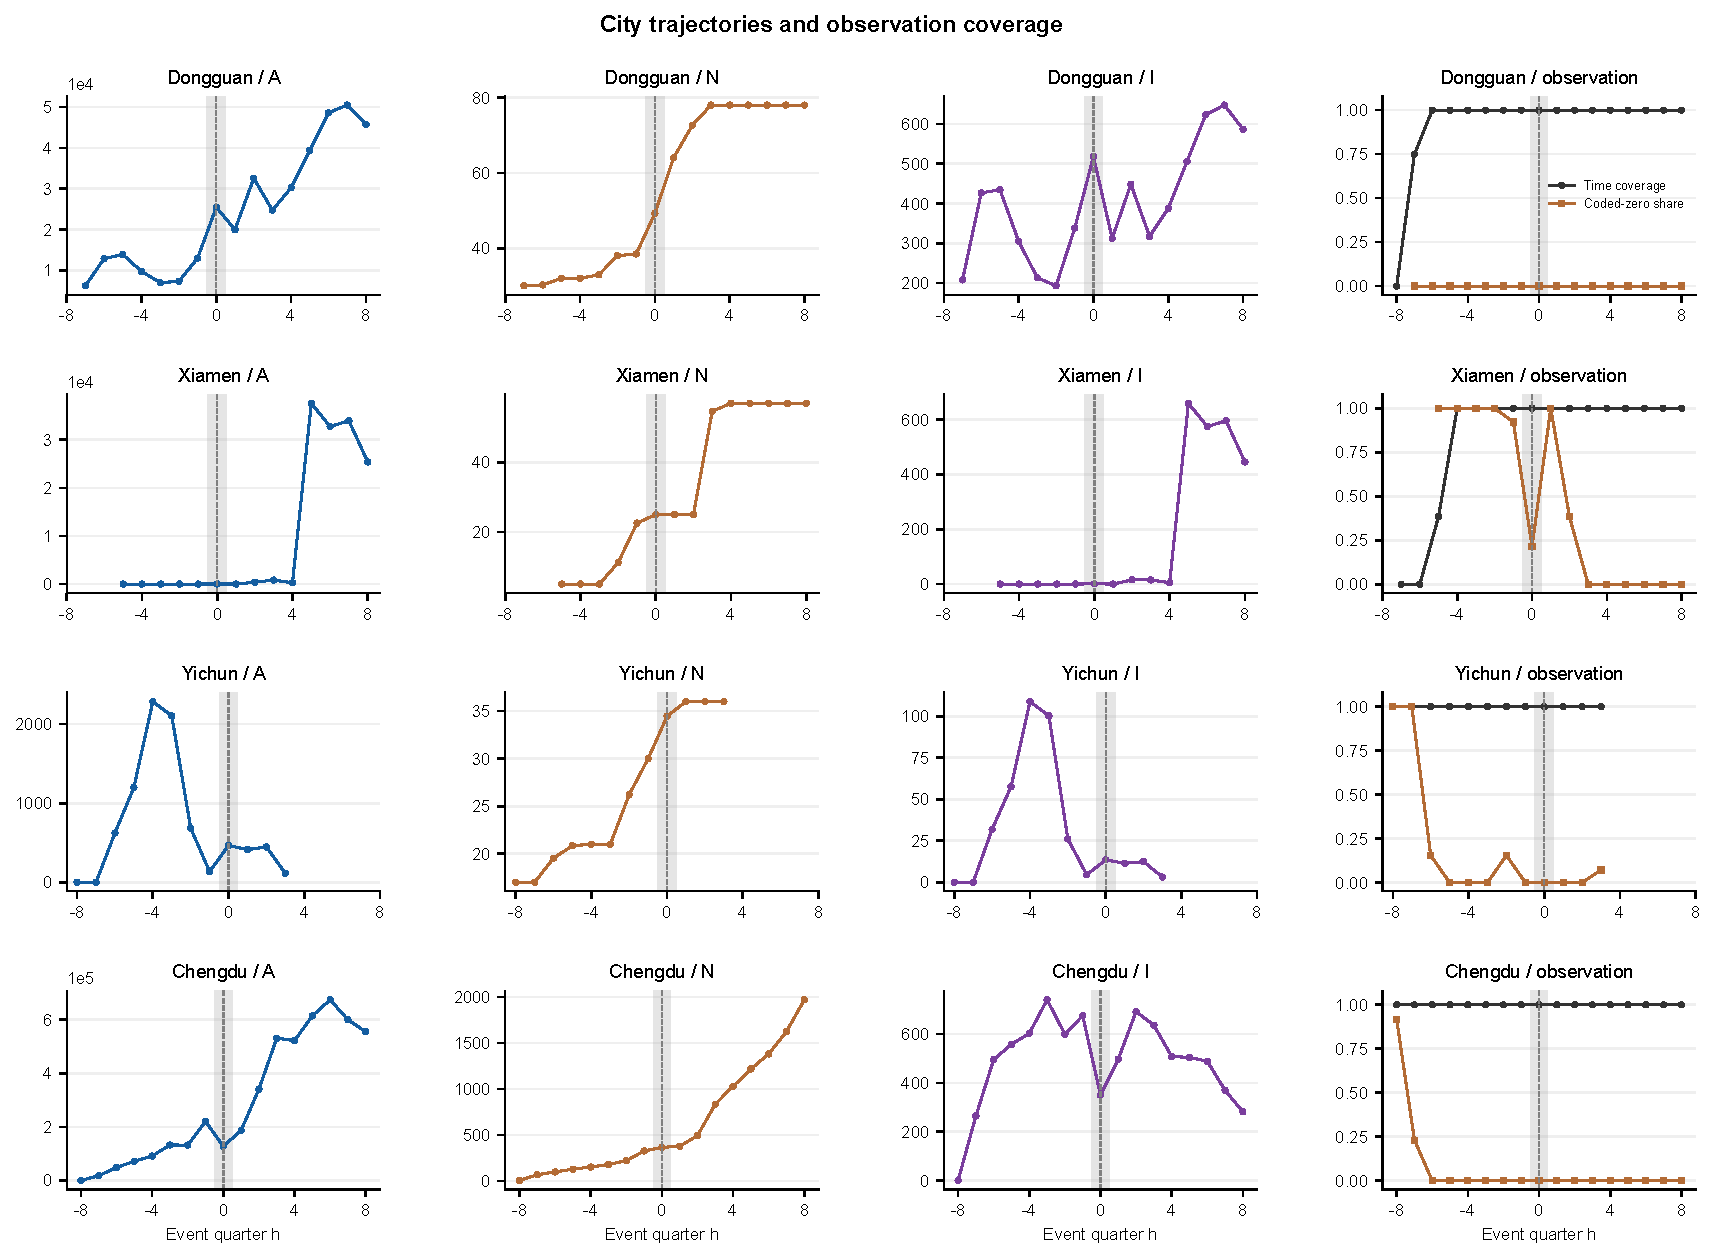
\includegraphics[width=\linewidth,height=.78\textheight,keepaspectratio]{figures/figS_city_paths_1.pdf}\captionof{figure}{City outcome paths and observation states, group 1}\label{fig:si_city_paths_1}\end{center}
\clearpage\begin{center}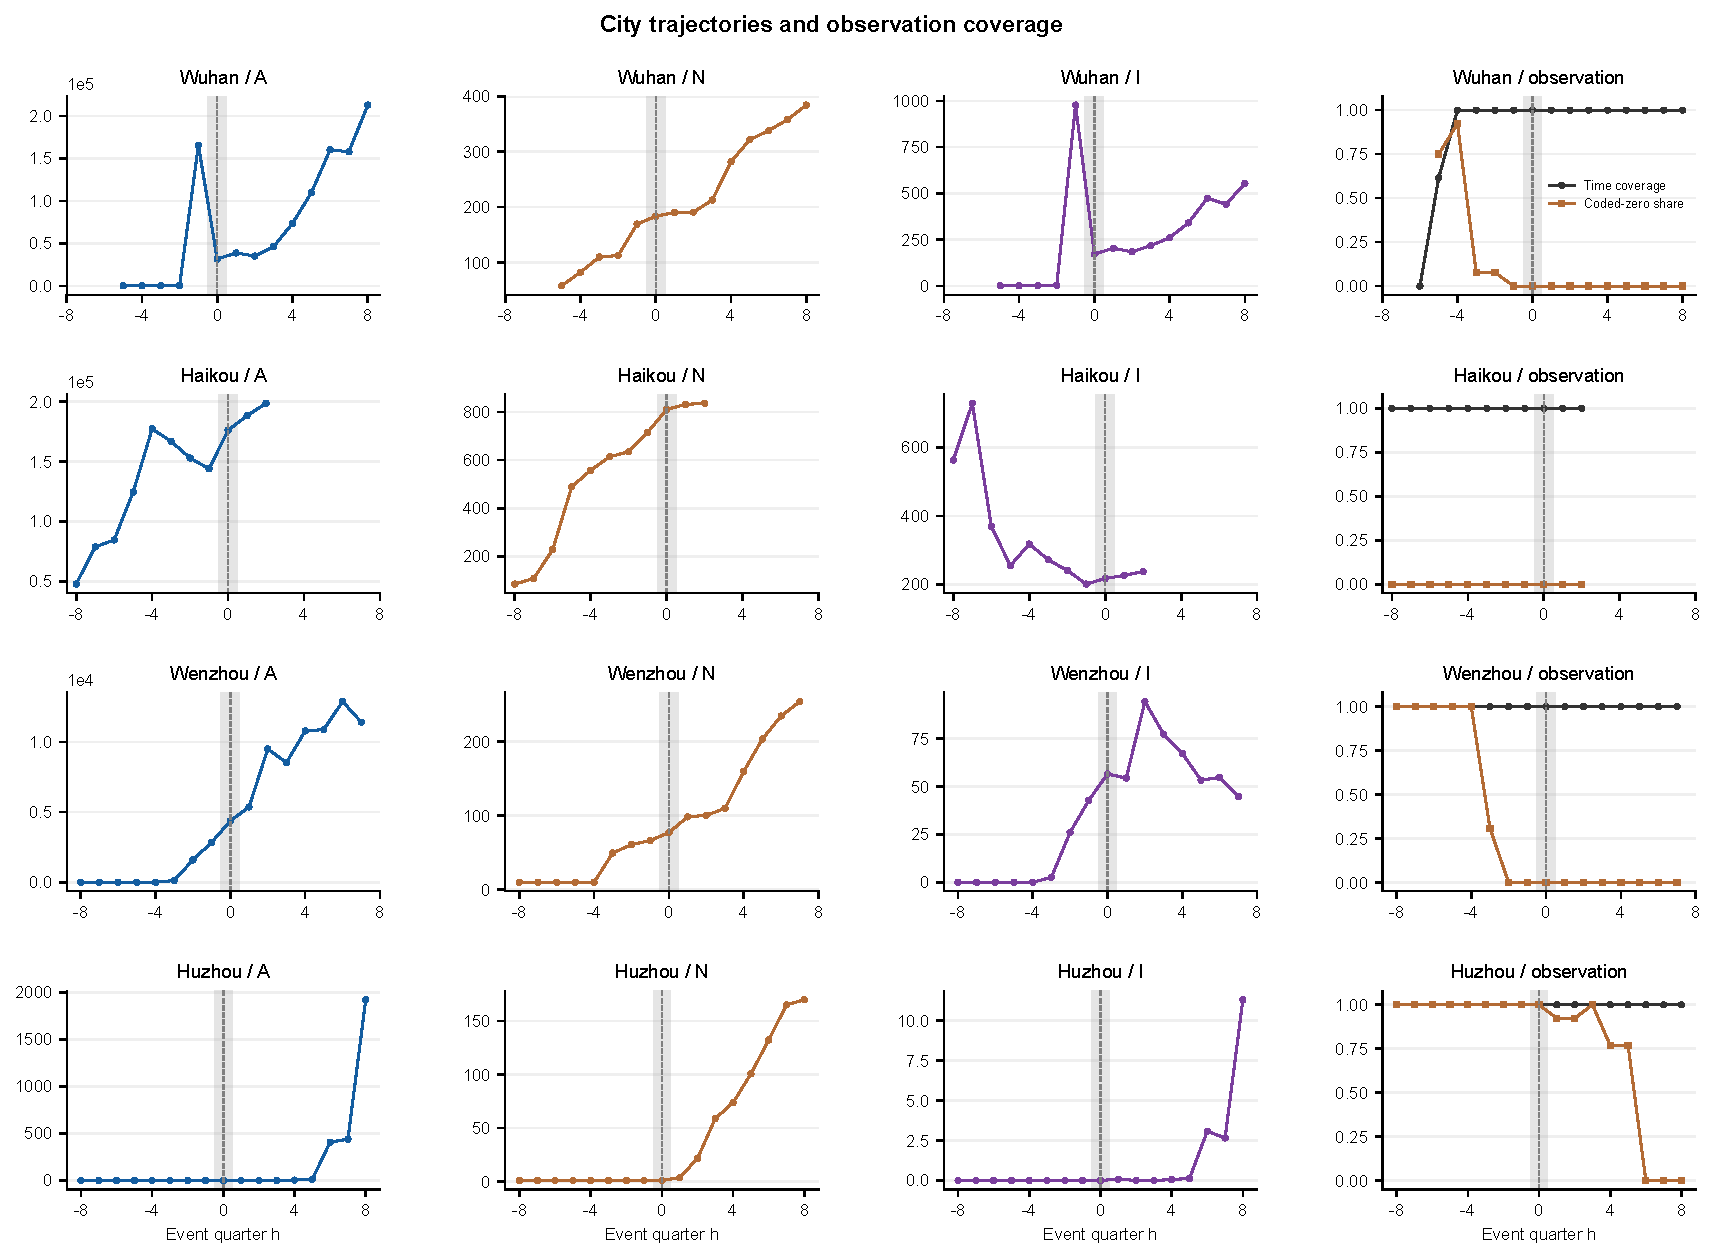
\includegraphics[width=\linewidth,height=.78\textheight,keepaspectratio]{figures/figS_city_paths_2.pdf}\captionof{figure}{City outcome paths and observation states, group 2}\label{fig:si_city_paths_2}\end{center}
\clearpage\begin{center}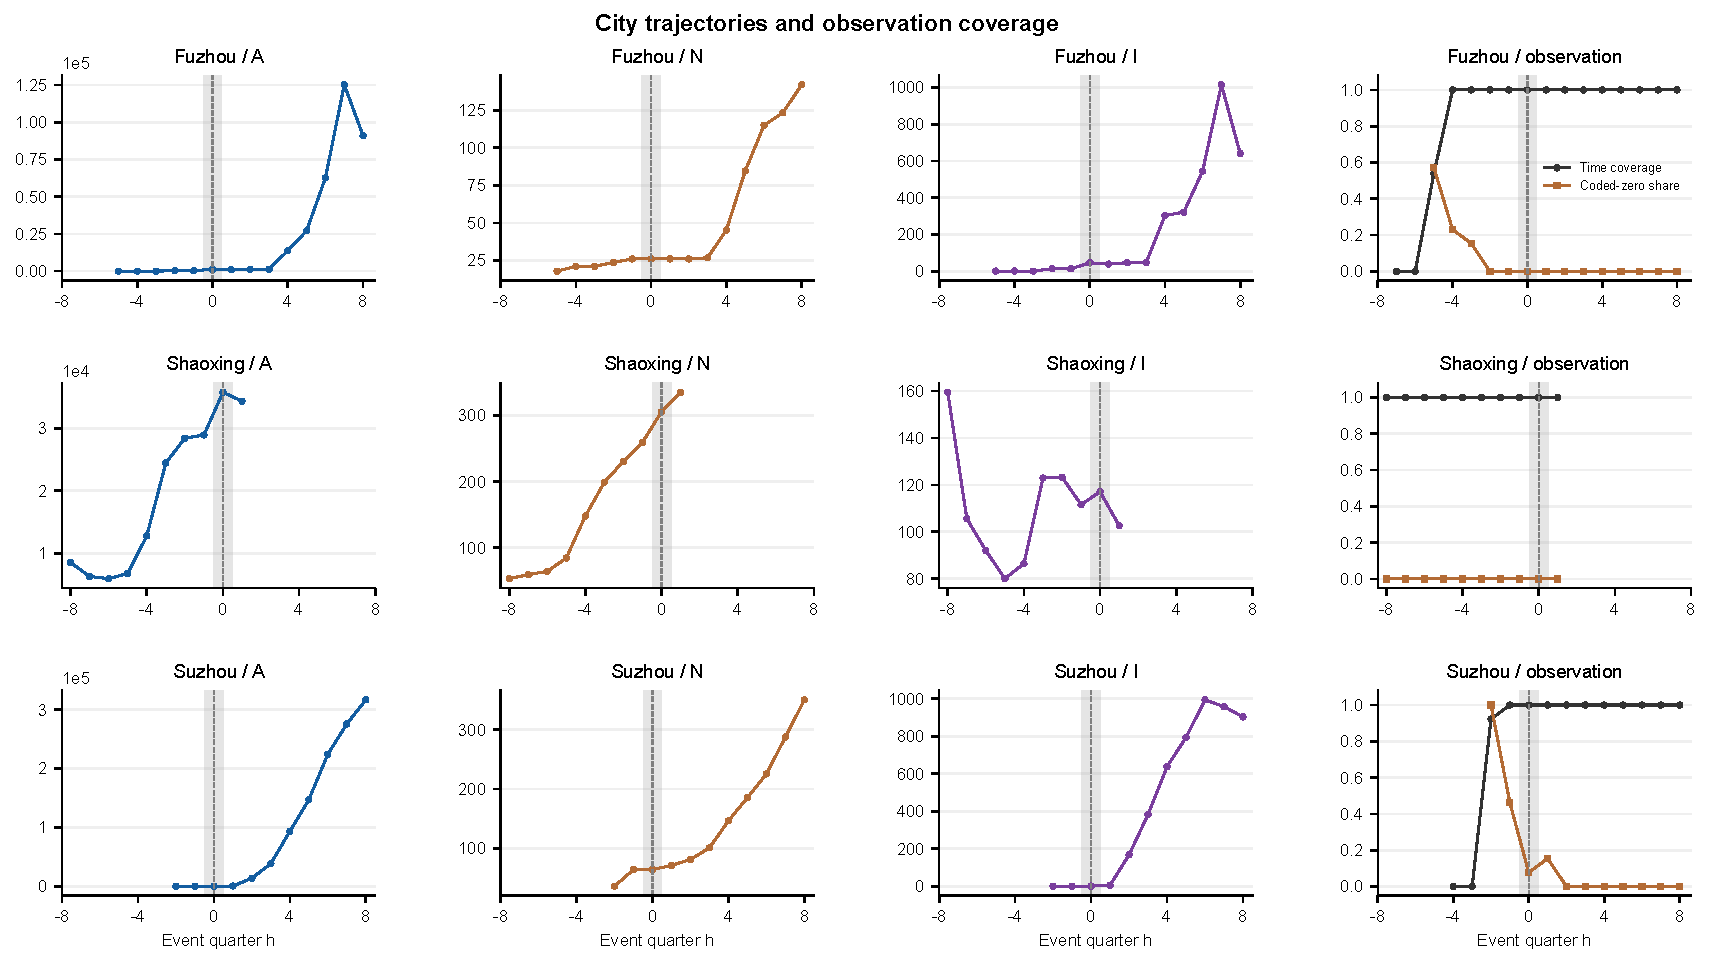
\includegraphics[width=\linewidth,height=.78\textheight,keepaspectratio]{figures/figS_city_paths_3.pdf}\captionof{figure}{City outcome paths and observation states, group 3}\label{fig:si_city_paths_3}\end{center}
